\documentclass[a4paper]{IEEEtran}

\usepackage{xcolor}
\usepackage{hyperref}
\usepackage[utf8]{inputenc}
\usepackage[pdftex]{graphicx} 

\newcommand\TODO[1]{\textcolor{red}{TODO:#1}}
\newcommand\todo[1]{\TODO{#1}}
\newcommand\cn{\textcolor{red}{[citation needed]}}

\title{The overpowered prefetcher of goodness and excellence!}

\author{
    Sigve Sebastian Farstad,
    Rune Holmgren,
    Torbjørn Langland,
    Per Thomas Lundal
}

\begin{document}

\maketitle

\begin{abstract}
    Le abstract.\cn
\end{abstract}

\section{Introduction}

\todo{ Write briefly about the project, the course it belongs to and the goal}
This is the introduction section.
Here we write something appealing for you to continue on.
If you finish this, you will be baked a cake.

As part of the course TDT4260 Computer Architecture, students in groups of 3 or 4 were to implement and test a prefetcher.
This report describes the implementation with test results done by group 11.
The report will describe the framework for the project, different prefetchers that have been implemented, how they work and the test results.

\section{Related Work}

\todo{ Not sure, mention related work?}
Here we mention related work. Do you want cake for your relatives?

\section{Prefetcher Description}
A total of 5 different prefetchers have been implemented and tested. 

\subsection{Delta correlation prediction table}

\subsection{Adaptive program counter delta correlation}

\subsection{Program counter c-zones delta correlation}

\subsection{C-zones delta correlation}

\subsection{Adaptive c-zones delta correlation}

\todo{Describe how the final prefetcher works. I suggest adding a figure. Maybe briefly mention other attempts while if we have space?}

\begin{figure}[h!]
  \centering
      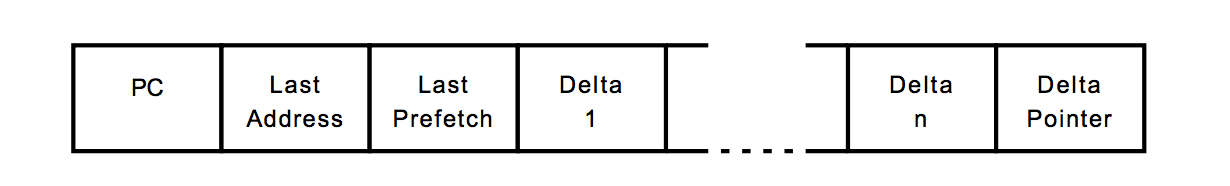
\includegraphics[width=0.5\textwidth]{Figures/DCTable}
  \caption{Delta Correlation Prediction Table}
  \label{fig:DCTable}
\end{figure}

Figure \ref{fig:DCTable} shows the Delta Correlation Prediction table used by the Prefetcher.
As can be seen, the a row in the table contains fields for the PC, last address, last prefetch, deltas 1 to n, and delta pointer.
PC stores the address to the load instruction, and works as index in the table.
The Last Address stores the missed address when there is a miss in the cache.
The delta fields stores the address difference, or the deltas, for each time this instruction is called.
By using the pattern in these deltas, one may predict the next loads, and thus issue prefetches based on the pattern.
An example would be the deltas 1, 2, 4, 1, 2, 4, ..., where 1, 2, 4, is repeated, and prefetches on addresses with these deltas in between may be issued.
Last prefetch contains the address of the last issued prefetch.
The Delta Pointer points to the head (first Delta field) in the row, since the delta fields are used as circular buffer.

\todo{There is more to be written, and current contents is... a bit poorly written}

\begin{figure}[h!]
  \centering
      
\includegraphics[width=0.5\textwidth]{Figures/DCExample}
  \caption{Delta Correlation Example}
  \label{fig:DCExample}
\end{figure}

Figure \ref{fig:DCExample} shows an example where the beginning load address is 10, with the deltas 1,9 in repeating pattern, and the addresses are 11, 20, 21, 30. 
\todo{ Write how this will work in the DCPT table}.


Here we describe the cake...uh, I mean the pretecher. Hey, Vance! Can you prefetch that cake?

\section{Methodology}

\todo{Mention the framework. Explain PFJudge. Maybe or maybe not mention C++?}
Here we describe how we did it.

WARNING: Recipee too long. Insert cake recipe here!

\section{Results}

\todo{ Describe results from both local and PFJudge.}

EXPLOSION!

\section{Discussion}

\todo{ Not exactly sure, just say it works better? Compare with other prefetcher IF we chose to describe them. }

You killed GLaDOS.
You monster.

\section{Conclusion}

\todo{ Mention what could have been done better or different? Future ideas? }

The cake is a lie!

\section{Acknowledgements (optional)}

GLaDOS

yoyo \cite{assignment-text}

\bibliography{bibliography}
\bibliographystyle{plain}
\nocite{*}

\end{document}
